% Copyright (C) 2024 - Michaël Baudin

\documentclass[9pt]{beamer}

%\setbeameroption{hide notes}
%\setbeameroption{show notes}
%\setbeameroption{show only notes}

% Copyright (C) 2012 - EDF R&D - Michael Baudin

% To highlight source code
\usepackage{listings}
\definecolor{darkgreen}{rgb}{0,0.5,0}
\definecolor{violet}{rgb}{0.5,0,1}

% \usepackage{lmodern}% http://ctan.org/pkg/lm

\usetheme{Darmstadt} % http://tex.stackexchange.com/questions/177042/beamer-latex-customized-formats

\useoutertheme[subsection=false,footline=authortitle]{miniframes}
% RGB scaled on 0-255 scale (section 17.1.1), colors pulled from title block
\usecolortheme[RGB={44, 131, 82}]{structure}

% hide header:
\setbeamertemplate{headline}{}

\usepackage[utf8]{inputenc}
\usepackage[T1]{fontenc}

%\usepackage[french]{babel}
%\uselanguage{French}
%\languagepath{French}

\def\bx{{\bf x}}
\def\RR{\mathbb{R}}

\newcommand{\pyvar}[1]{\texttt{#1}}

\def \ot {OpenTURNS}

\hypersetup{colorlinks=true}

\lstset{
  % general command to set parameter(s)
   %basicstyle=\footnotesize\ttfamily, %
   %basicstyle=\normalsize \ttfamily, %
   basicstyle=\scriptsize\ttfamily, %
   keywordstyle=\color{violet}\bfseries,%
   commentstyle=\color{darkgreen}\bfseries,%
   showspaces=false,%
   stringstyle=\color{red}\bfseries, 
   otherkeywords={Gumbel, TruncatedDistribution, LatentVariableModel, %
        SmoothedUniformFactory, Uniform, PythonFunction, ComposedDistribution, %
        StudentCopula, StudentCopulaFactory, RankSobolSensitivityAlgorithm, %
	   MonteCarlo, IntervalMesher, PointToFieldFunctionalChaosAlgorithm, FieldFunctionalChaosSobolIndices, HistogramFactory, %
	   Graph, BoxCoxFactory, CompositeProcess, WhittleFactory, ARMAFactory, %
	   Basis, TrendFactory, BoxCoxTransform, SpatialFunction, TimeSeries, %
	   WelchFactory, GreaterOrEqual, IndependentCopula, %
	   SystemFORM, UnionEvent, IntersectionEvent},
}


\title[Calibration in OpenTURNS]{Overview of calibration features in OpenTURNS}

\author[M. Baudin]{
Michaël Baudin \inst{1}
}

\institute[EDF]{
\inst{1} EDF R\&D. 6, quai Watier, 78401, Chatou Cedex - France, michael.baudin@edf.fr
}


\date[]{June 19th 2024, Palaiseau, France}


%%%%%%%%%%%%%%%%%%%%%%%%%%%%%%%%%%%%%%%%%%%%%%%%%%%%%%%%%%%%%%%%%%%%%%%%%%%%%

\begin{document}

%%%%%%%%%%%%%%%%%%%%%%%%%%%%%%%%%%%%%%%%%%%%%%%%%%%%%%%%%%%%%%%%%%%%%%%%%%%%%

\begin{frame}
\titlepage

\begin{center}

\includegraphics[height=0.15\textheight]{figures/edf.jpg}
\end{center}

\end{frame}

%%%%%%%%%%%%%%%%%%%%%%%%%%%%%%%%%%%%

\begin{frame}
\frametitle{Introduction}

Calibration is the step B' of the generic methodology\footnote{See\cite{Baudin2016, BaudinMethodes2020}.}.

\begin{figure}
\begin{center}
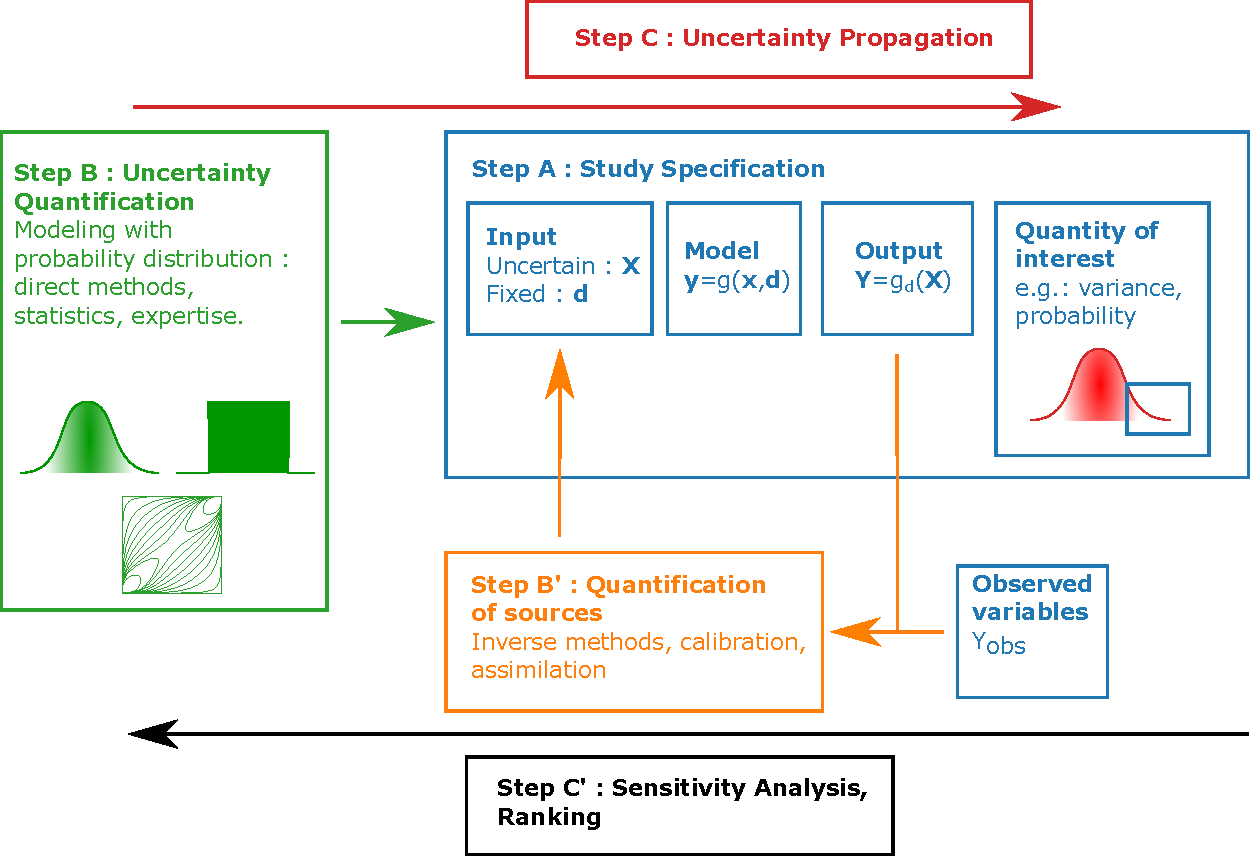
\includegraphics[width=0.7\textwidth]{MethodologieIncertitude-EN.pdf}
\end{center}
\caption{The step B' brings the observed predictions from the model
closer to the observed outputs to calibrate the parameters.}
\end{figure}

\end{frame}

%%%%%%%%%%%%%%%%%%%%%%%%%%%%%%%%%%%%

\begin{frame}
\frametitle{Introduction}

We have:
\begin{itemize}
\item a dataset,
\item a parametric model with unknown parameters.
\end{itemize}

We search for:
\begin{itemize}
\item parameter values,
\item such that the predictions of the model are as close as possible to the data.
\end{itemize}

Since the dataset is random, we want the distribution of the parameters.

From there, we can compute confidence intervals of the parameters.

\begin{figure}
\begin{center}
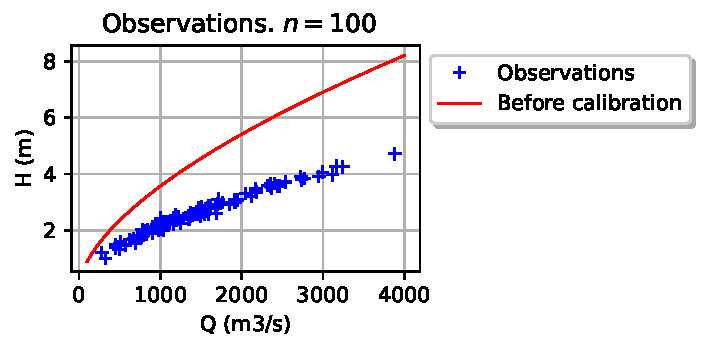
\includegraphics[width=0.5\textwidth]{flooding_before_calibration.pdf}
\end{center}
\caption{Observations compared to the predictions of a model.}
\end{figure}

\end{frame}

%%%%%%%%%%%%%%%%%%%%%%%%%%%%%%%%%%%%

\begin{frame}[fragile]
\section{Overview}
\frametitle{Overview}

In OpenTURNS, we have several calibration features:
\begin{itemize}
\item \href{https://openturns.github.io/openturns/latest/theory/data_analysis/data_analysis.html#calibration}{theory help pages}
\item \href{https://openturns.github.io/openturns/latest/user_manual/calibration.html}{API help pages}
\item \href{https://openturns.github.io/openturns/latest/auto_calibration/index.html}{examples}.
\end{itemize}


There are two types of features :
\begin{itemize}
\item linear and non linear least squares, Gaussian linear and non linear calibration : \pyvar{*Calibration} classes. These classes compute the \textbf{posterior distribution of the parameters}.
\item Monte Carlo Markov Chain (MCMC) algorithms : \pyvar{*MetropolisHastings}, etc. These classes \textbf{generate a sample from the posterior distribution of the parameters}.
\end{itemize}

The simplest example is \href{https://openturns.github.io/openturns/latest/auto_calibration/least_squares_and_gaussian_calibration/plot_calibration_quickstart.html#sphx-glr-auto-calibration-least-squares-and-gaussian-calibration-plot-calibration-quickstart-py}{Calibrate a parametric model: a quick-start guide to calibration}

Here, we are going to review the \href{https://openturns.github.io/openturns/latest/auto_calibration/least_squares_and_gaussian_calibration/plot_calibration_flooding.html#sphx-glr-auto-calibration-least-squares-and-gaussian-calibration-plot-calibration-flooding-py}{Calibration of the flooding model}
\end{frame}


%%%%%%%%%%%%%%%%%%%%%%%%%%%%%%%%%%%%

\begin{frame}[fragile]
\section{Conclusion}
\frametitle{Conclusion}

Other tools :
\begin{itemize}
\item Calibration methods are also available in \href{https://persalys.fr}{Persalys} : linear and non linear least squares, Gaussian linear and non linear calibration.
\end{itemize}

Perspectives:
\begin{itemize}
\item provide bounds to the optimization algorithms (return truncated normal distribution if necessary);
\item unify the \pyvar{ParametricFunction} in \pyvar{*Calibration} and \pyvar{*MetropolisHastings} classes (exchange the roles of $x$ and $\theta$);
\item calibrate parametric functions with field output more easily;
\item provide algorithms to automatically compute finite difference steps (not specific to calibration);
\item provide the covariance matrix of the parameters as a diagonal matrix when possible;
\item scale the parameters to calibrate (not specific to calibration);
\item implement \pyvar{CalibrationResult.isBayesian()} (see \href{https://github.com/openturns/openturns/issues/2560}{2560});
\item implement a \pyvar{CalibrationResult} structure for M.-H. classes.
\end{itemize}
\end{frame}



%%%%%%%%%%%%%%%%%%%%%%%%%%%%%%%%%%%%

\section{References}
\begin{frame}[allowframebreaks]
\frametitle{Références}
\nocite{*}
\bibliographystyle{apalike}
\bibliography{calibration2024}
\end{frame}

\end{document}
